\documentclass{article}

\usepackage{graphicx}
\usepackage{float}
\graphicspath{ {./images/} }

\title{Scalar Spherical Harmonics and Slepian Functions}
\author{H. A. Werth}
\date{}


\setlength{\parskip}{0.5cm plus4mm minus3mm}

\textwidth=6.4in
\textheight=8.5in
\hoffset=-0.7in
\voffset=-0.7in

\setlength{\parindent}{0cm} 


\begin{document}
\maketitle

\tableofcontents 

\section{Plot a single spherical harmonic function}

We will demonstrate plotting a spherical-harmonic on a sphere,  in a standard Matlab plot, on a Mollweide projection, and on random points of a sphere.

First, designate a spherical-harmonic to be plotted:

For example,

\verb+l+ = 3; \verb+m+ = -2;

0 ≤ \verb+l+ fixes the degree and \verb+m+ fixes the order.

\subsection{Plot on sphere}

Example:
\vspace{2mm}

\setlength{\parskip}{.1mm}

\verb+l+ = 3; \verb+m+ = -2;

\verb+lon = 0:0.5:360;+

\verb+lat = -90:0.5:90;+

\verb+Y = ylm(l, m, pi/180*(90-lat), pi/180*lon);+

\verb+figure;+

\verb+plotplm(Y, pi/180*lon, pi/180*lat,2)+

\begin{figure}[H]
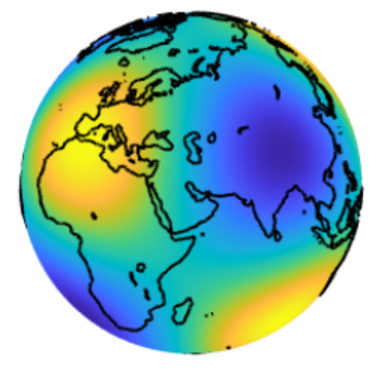
\includegraphics[scale=1]{graph_on_sphere}
\end{figure}

\setlength{\parskip}{0.5cm plus4mm minus3mm}

1. Create a grid on the sphere

\verb+lon = 0:0.5:360;+
\verb+lat = -90:0.5:90;+

This creates a coordinate point every half-degree.

2. Calculate the values of the function for coordinate points on the sphere

\verb+Y = ylm(l, m, pi/180*(90-lat), pi/180*lon);+

The function \verb+slepian_alpha/ylm.m+ evaluates the spherical harmonic function of degree \verb+l+ and order \verb+m+ at every point \verb+pi/180*(90-lat)+, \verb+pi/180*lon+ on the grid. We name the vector of the spherical-harmonic values “\verb+Y+”.

Note that \verb+90-lat+ is needed to convert latitude to colatitude and \verb+pi/180+ is needed to convert degrees to radians.

3. Plot

\verb+figure;+
\verb+plotplm(Y, pi/180*lon, pi/180*lat,2)+

The function \verb+slepian_alpha/plotplm.m+ is here used to plot the vector \verb+Y+ using the grid specified by “\verb+lon+” and “\verb+lat+” in step 1. The input \verb+2+ dictates that the graph be on a sphere.

\subsection{Plot in standard Matlab plot}

Example:
\vspace{2mm}

\setlength{\parskip}{.1mm}

\verb+l+ = 3; \verb+m+ = -2;

\verb+lon = 0:0.5:360;+

\verb+lat = -90:0.5:90;+

\verb+Y = ylm(l, m, pi/180*(90-lat), pi/180*lon);+

\verb+imagesc(lon, lat, Y)+

\begin{figure}[H]
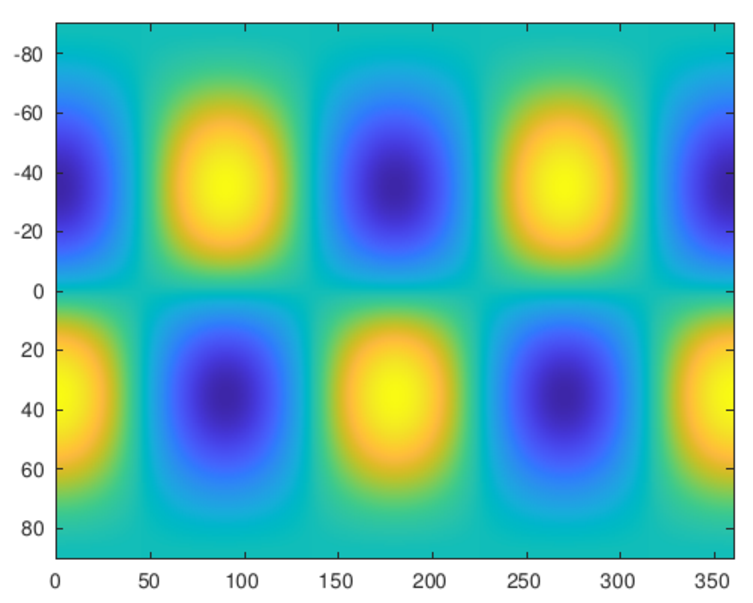
\includegraphics[scale=.6]{standard_matlab_plot}
\end{figure}

\setlength{\parskip}{0.5cm plus4mm minus3mm}

Do steps 1 and 2, and then run

\verb+imagesc(lon, lat, Y)+

\subsection{Plot on Mollweide projection}

Example:
\vspace{2mm}

\setlength{\parskip}{.1mm}

\verb+l+ = 3; \verb+m+ = -2;

\verb+lon = 0:0.5:360;+

\verb+lat = -90:0.5:90;+

\verb+Y = ylm(l, m, pi/180*(90-lat), pi/180*lon);+

\verb+figure;+

\verb+plotplm(Y, pi/180*lon, pi/180*lat,1)+

\begin{figure}[H]
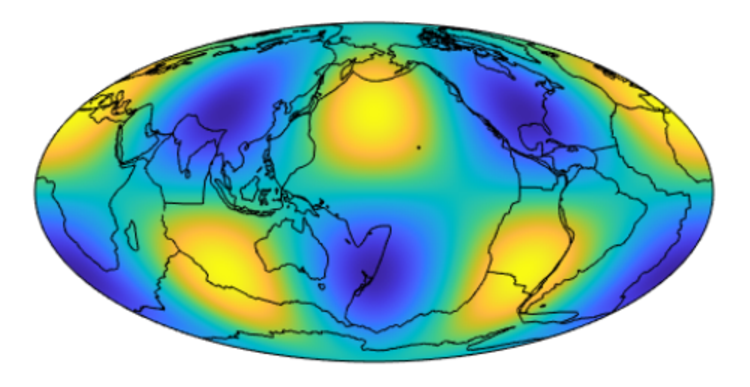
\includegraphics[scale=.8]{mollweide}
\end{figure}

\setlength{\parskip}{0.5cm plus4mm minus3mm}

Do steps 1 and 2, and then run

\verb+figure;+

\verb+plotplm(Y, pi/180*lon, pi/180*lat,1)+

The input \verb+1+ dictates that the graph be on the Mollweide projection.

\subsection{Plot for random points on a sphere}

Example:
\vspace{2mm}

\setlength{\parskip}{.1mm}

\verb+l+ = 3; \verb+m+ = -2;

\verb+TH = 120; lon0 = 30; cola0 = 40; N=1000;+

\verb+[lon, lat] = randpatch(N,TH,lon0,cola0);+

\verb+Y = ylm(l, m, pi/180*(90-lat), pi/180*lon,[],[],[],1);+

\verb+scatter(lon, lat, [], Y)+

\begin{figure}[H]
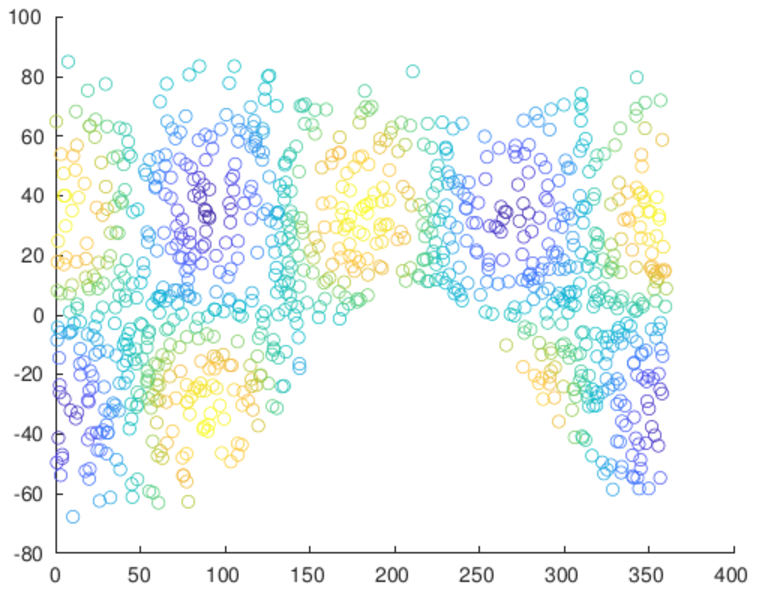
\includegraphics[scale=.75]{random_plot}
\end{figure}

\setlength{\parskip}{0.5cm plus4mm minus3mm}

1. Generate a subset of the sphere consisting of random points 

In particular, we will create \verb+N+ randomly-generated coordinate points within a spherical cap of opening angle \verb+TH+ and centered at longitude \verb+lon0+ and colatitude \verb+cola0+

For example, 

\verb+TH = 120; lon0 = 30; cola0 = 40; N=1000;+

\verb+[lon, lat] = randpatch(N,TH,lon0,cola0);+

The function \verb+slepian_alpha/randpatch.m+ creates the set of random points within the spherical cap of the specified values. We name those coordinate points \verb+[lon,lat]+.

2. Calculate the values of the spherical harmonic at those points

\verb+Y = ylm(l, m, pi/180*(90-lat), pi/180*lon,[],[],[],1);+


\verb+ylm.m+ takes the arguments \verb+l+, \verb+m+, \verb+pi/180*(90-lat)+, \verb+pi/180*lon+ as before. Run \verb+help ylm+ for information on all eight arguments. 

3. Plot

If necessary, use the Matlab command 

\verb+ clf;+

To clear existing figures, and then run the Matlab command

\verb+scatter(lon, lat, [], Y)+

To create a scatter plot of circles having locations \verb+[lon, lat]+. Here, \verb+[]+ indicates the default value for circle size and the vector of spherical-harmonic values \verb+Y+ is used to determine circle color. 

Please see \verb+Ch_01+ in the \verb+.edu+ folder for more detailed information.

\section{Plot a linear combination of spherical harmonics}

Example:
\vspace{2mm}

\setlength{\parskip}{.1mm}

\verb+lon = 0:0.5:360;+

\verb+lat = -90:0.5:90;+

\verb+Y1=ylm(3,1,pi/180*(90-lat),pi/180*lon);+

\verb+Y2=ylm(1,-1,pi/180*(90-lat),pi/180*lon);+

\verb+Y3=ylm(5,-2,pi/180*(90-lat),pi/180*lon);+

\verb!Y4=4*Y1-0.2*Y2+2*Y3;!

\verb+plotplm(Y4, pi/180*lon, pi/180*lat,1);+

\verb!kelicol(1)!
\begin{figure}[H]
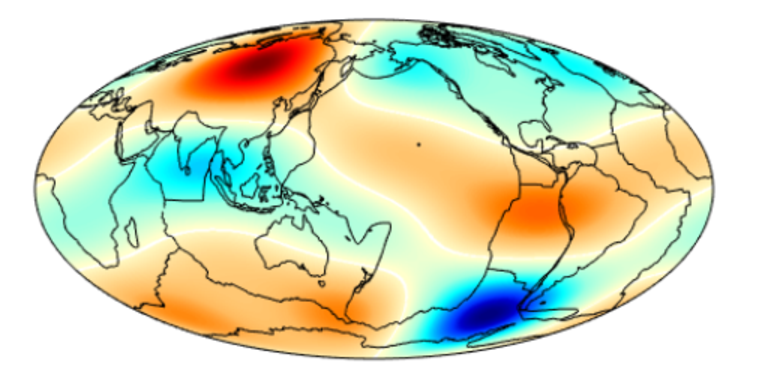
\includegraphics[scale=1]{linear_combination}
\end{figure}

\setlength{\parskip}{0.5cm plus4mm minus3mm}

This task is a simple variation on the first. 

Let us define three spherical harmonics:

\verb+lon = 0:0.5:360;+

\verb+lat = -90:0.5:90;+

\verb+Y1=ylm(3,1,pi/180*(90-lat),pi/180*lon);+

\verb+Y2=ylm(1,-1,pi/180*(90-lat),pi/180*lon);+

\verb+Y3=ylm(5,-2,pi/180*(90-lat),pi/180*lon);+

Next, create a vector which is a linear combination of these three. For example,

\verb!Y4=4*Y1-0.2*Y2+2*Y3;!

To plot the function, use \verb+plotplm.m+. For example,

\verb+plotplm(Y4, pi/180*lon, pi/180*lat,1)+

If you're interested in another color scheme, try out 

\verb+kelicol(1)+

Please see \verb+Ch_01+ in the \verb+.edu+ folder for more detailed information.

\section{Create and plot scalar Slepian functions}

\subsection{Named region and polar cap}

Named region example 1:

\vspace{2mm}

\setlength{\parskip}{.1mm}

\verb![G] = glmalpha('africa',20,[],0);!

\verb!lmcs = coef2lmcosi(G(:,1),1);!

\verb!data=plm2xyz(lmcs,0.5);!

\verb!plotplm(data, [], [], 1, 0.5)!

\begin{figure}[H]
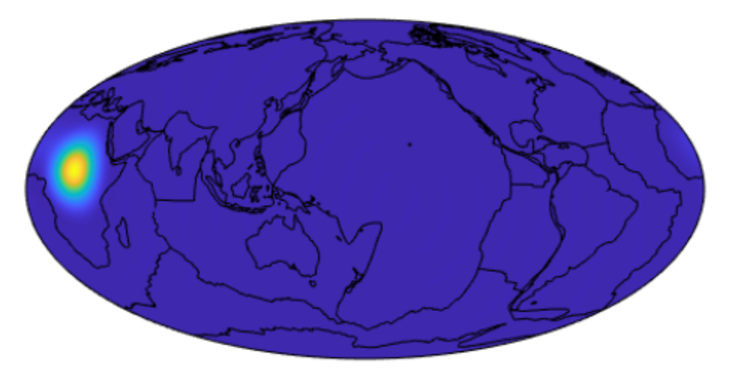
\includegraphics[scale=.75]{africa_ex_1}
\end{figure}

\setlength{\parskip}{0.5cm plus4mm minus3mm}

Named region example 2:

\vspace{2mm}

\setlength{\parskip}{.1mm}

\verb![G] = glmalpha('england',20,[],0);!

\verb!lmcs = coef2lmcosi(G(:,3),1);!

\verb!data=plm2xyz(lmcs,0.5);!

\verb!plotplm(data, [], [], 2, 0.5)!

\begin{figure}[H]
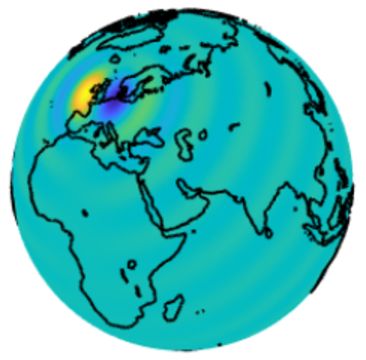
\includegraphics[scale=1.2]{england_ex_2}
\end{figure}

\setlength{\parskip}{0.5cm plus4mm minus3mm}

Polar cap example:

\vspace{2mm}

\setlength{\parskip}{.1mm}

\verb![G] = glmalpha(40,20,1,0)!

\verb!lmcs = coef2lmcosi(G(:,1),1);!

\verb!data=plm2xyz(lmcs,0.5);!

\verb!plotplm(data, [], [], 2, 0.5)!

\verb!view(2)!

\begin{figure}[H]
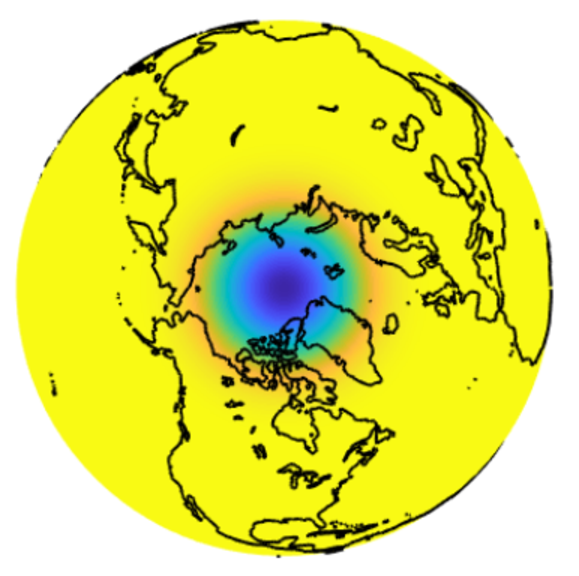
\includegraphics[scale=.75]{polarcap_ex}
\end{figure}

\setlength{\parskip}{0.5cm plus4mm minus3mm}

To create the Slepian function to be plotted is to generate its spherical-harmonic coefficients. For this task we will use  the function \verb!glmalpha.m!, which computes the best spatially-concentrated Slepian functions given two constraints. Those constraints are the first input, \verb!TH!, either a named region or the opening angle in degrees of a polar cap, and the second, \verb!L!, the bandwidth. The named regions recognized by \verb!glmalpha! are 'england', 'eurasia',  'namerica', 'australia', 'greenland', 'africa', 'samerica', 'amazon', 'orinoco', 'antarctica', 'contshelves', and  'alloceans'.

For example, 

\verb![G] = glmalpha('africa',20,[],0);!


\verb![G]! is a matrix whose $n$th column holds the coefficients of the $n$th-best spatially-concentrated Slepian function. In order to plot the $n$th function we need to convert the $n$th column of \verb![G]! into the form recognized by the function \verb!plotplm.m!, the so-called "lmcosi" format.

\verb!lmcs = coef2lmcosi(G(:,1),1);!

Here we have chosen to use the first column \verb!G(:,1)!. The second input \verb!1! is necessary when the coefficients are calculated using \verb!glmalpha!.

Now we input the (lmcosi-formatted) matrix \verb!lmcs! and a resolution into the function \verb!plm2xyz!. We choose the resolution to be 0.5 and name the ouput "data":

\verb!data=plm2xyz(lmcs,0.5);!

\vspace{3mm}

Now to plot, run

\verb!plotplm(data, [], [], 1, 0.5)!

The input \verb!1! specifies Mollweide projection and the input \verb!0.5! is just the resolution again.

The same sequence is used to plot a Slepian function on a polar cap, except for a change in the inputs to \verb!glmalpha.m! Specifically, we will now let \verb!TH! denote an opening angle in degrees.

For example, let \verb!TH = 40!.

\verb![G] = glmalpha(40,20,2,0)!

The command 

\verb!view(2)!

may be used to rotate the spherical figure so that the North pole is faced toward the viewer.

We suggest reading the \verb!help! section for the relevant functions and/or Chapter 2, Section 1 in the folder \verb!.edu! for a detailed discussion.

\subsection{Rotated polar cap}

Example:

\vspace{3mm}

\setlength{\parskip}{.1mm}

\verb![G] = glmalphaptoJ(40,20,180,45,0,10)!

\verb!lmcs = coef2lmcosi(G(:,1),1);!

\verb!data=plm2xyz(lmcs,0.5);!

\verb!plotplm(data, [], [], 1, 0.5)!


\begin{figure}[H]
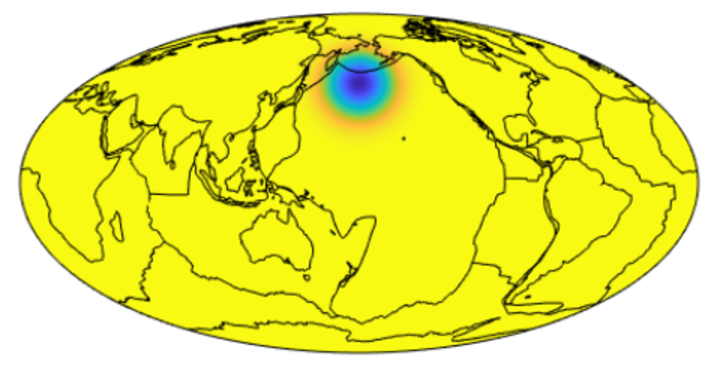
\includegraphics[scale=.75]{rotated_example}
\end{figure}

\setlength{\parskip}{0.5cm plus4mm minus3mm}

The general method of calculuating coefficients for a rotated polar cap is the same as above, but involves slightly different commands.

We will need to use the function \verb!glmalphaptoJ! and provide the following inputs:

\verb!TH!: opening angle

\verb!L!: maximum spherical harmonic degree (bandwidth)

\verb!phi!: longitude in degrees

\verb!theta!: colatitude in degrees

\verb!omega!: rotation of the region itself, if any

\verb!J!: number of Slepian functions to be calculated

\section{Compute spherical-harmonic coefficients from regional data}

Slepian functions may be used to represent data obtained from regional observations. The goal of the current task is to calculate the spherical-harmonic coefficients of the Slepian function which best represents such a data set.

In a preliminary step we create the "observations" from random spherical-harmonic coefficients. 

Example:

\vspace{3mm}

\setlength{\parskip}{.1mm}

\verb!N=5000!

\verb!dom='namerica'!

\verb![lon,lat]=randinpoly(dom,N);!

\verb!Lmax=20!

\verb!lmcosi=plm2rnd(Lmax,0)!

\verb!data = plm2xyz(lmcosi,lat,lon);!

\verb!subplot(2,1,1)!

\verb!scatter(lon,lat,[],data)!

\begin{figure}[H]
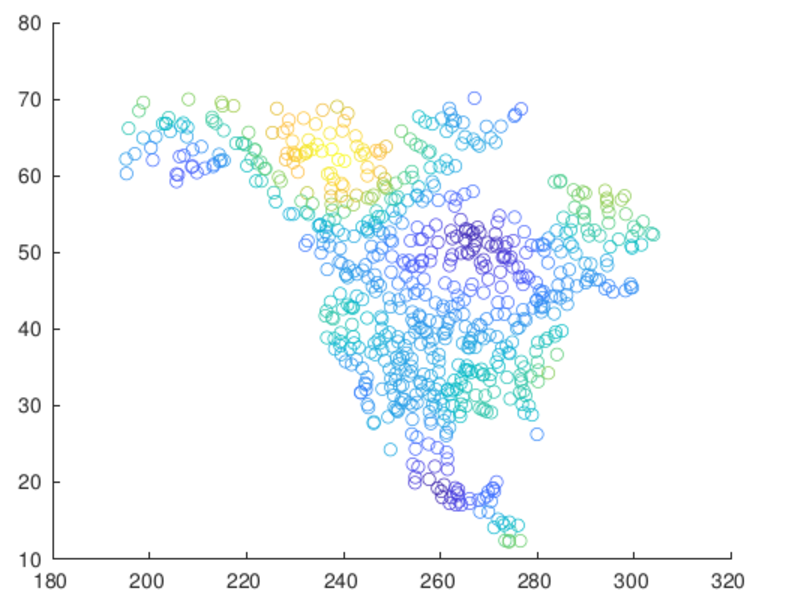
\includegraphics[scale=.75]{namerica_randomdata}
\end{figure}

\setlength{\parskip}{0.5cm plus4mm minus3mm}

The main task consists of obtaining the spherical-harmonic coefficients from the observations.

Example:

\vspace{3mm}

\setlength{\parskip}{.1mm}

\verb![G,V]=glmalpha(dom,Lmax);!

\verb!Y=ylm([0 Lmax],[],(90-lat)*pi/180,lon*pi/180+pi,[],[],[],1)!

\verb!J = min((Lmax+1)^2,round(1.5*(Lmax+1)^2*spharea(dom)));!

\verb!Geval = G(:,1:J)'*Y;!

\verb!gcoef = (Geval*Geval')\(Geval*data);!

\verb!coef = G(:,1:J)*gcoef;!

\verb!subplot(2,1,2)!

\verb!plotplm(coef2lmcosi(coef,1),[],[],4,1)!

\begin{figure}[H]
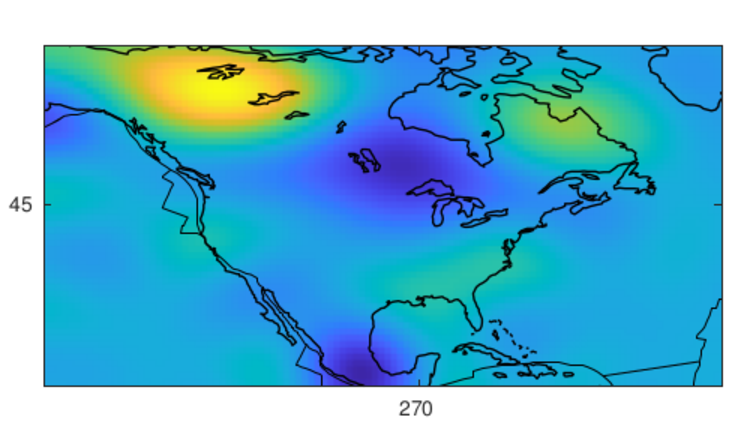
\includegraphics[scale=.75]{namerica_solvedcoefficients}
\end{figure}

\setlength{\parskip}{0.5cm plus4mm minus3mm}

Step 1.

First choose a region and create \verb!N! random data locations within the region. For example,

\verb!N=5000!

\verb!dom='namerica'!

\verb![lon,lat]=randinpoly(dom,N);!

Next, create random spherical-harmonic coefficients using the function \verb!plm2rnd.m!, which makes random coefficients for spherical harmonics up to degree \verb!L! and stores them in an \verb!lmcosi! matrix. For this example, let \verb!Lmax=L=20!.

\verb!Lmax=20!

\verb!lmcosi=plm2rnd(Lmax,0)!

Now evaluate the Slepian function determined by these random coefficients at these locations:

\verb!data = plm2xyz(lmcosi,lat,lon);!

To look at the data,

\verb!subplot(2,1,1)!

\verb!scatter(lon,lat,[],data)! 

\begin{figure}[H]
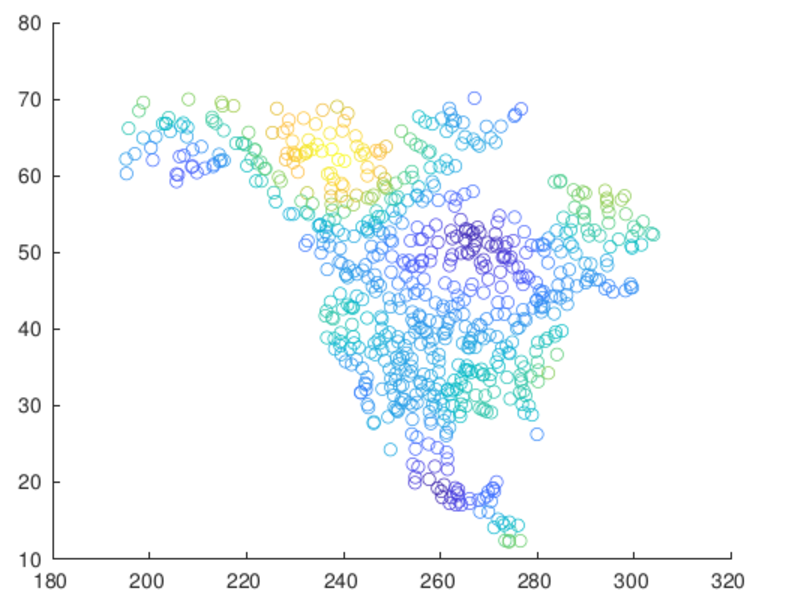
\includegraphics[scale=.6]{namerica_randomdata}
\end{figure}

Step 2.

We will now treat \verb!data! as a collection of observations and try to find the Slepian function which “best fits” the observations. We already know the function of best fit in this example; it is that whose spherical-harmonic coefficients are given in \verb!lmcosi! and whose values are the entries of \verb!data!. But be careful to note that \verb!data! only represents the values of that function $F$ over a subset of its domain, the randomly-generated \verb![lon,lat]! points in 'namerica'. The coefficients we will obtain in this Step will determine a Slepian function which matches $F$ on \verb![lon,lat]!, but which has no reason to coincide with it over the rest of the sphere. 

First, we will use \verb!glmalpha! to compute the coefficients of the best spatially-concentrated Slepian functions over our chosen region \verb!dom! and chosen bandwidth \verb!Lmax!. From this set of functions will be chosen the one which best fits \verb!data!.

\verb![G,V]=glmalpha(dom,Lmax);!

Evaluate the spherical harmonics of degrees \verb!0! to \verb!Lmax! at the data points:

\verb!Y=ylm([0 Lmax],[],(90-lat)*pi/180,lon*pi/180+pi,[],[],[],1)!

Next evaluate the Slepian functions at the data points. All of these evaluated Slepian functions are linear combinations of the above evaluated spherical harmonics; they differ by their coefficients, which are stored in the matrix \verb+[G]+. Therefore, in order to evaluate a Slepain function whose coefficients come from the $n$th vector of \verb+[G]+, we would run something like

\verb!eval=G(:,n)'*Y!

(Recall that \verb!transpose(A)=A' ! in Matlab.)

But we want to evaluate the  functions for the first \verb!J! vectors of \verb![G]! simultaneously, in order that we may compare them for best fit to \verb!data!, so we run

\verb!J = min((Lmax+1)^2,round(1.5*(Lmax+1)^2*spharea(dom)));!

\verb!Geval = G(:,1:J)'*Y;!

See that we have replaced the column argument “\verb+n+” with “\verb+1:J+”.

(This choice of \verb!J! should be sufficient in most situations. \verb!(Lmax+1)^2! is the number of Slepian functions which exist up to a maximum degree \verb!Lamx!, and \verb!spharea(dom)! is the area of the domain relative to the whole sphere. The role of these quantities in choosing \verb!J! was decided upon in order to optimize the solution to the linear system below relative to other factors like noise sensitivity. The scaling factor \verb!1.5! is usually a safe choice but varies with the context.)

To determine which of these \verb!J! functions best fits \verb!data!, we must solve for a vector \verb!gcoef! in

\verb!Geval*gcoef = data!

This is an over-determined system, so we use the least-squares method to compute \verb!gcoef!:

\verb!gcoef = (Geval*Geval')\(Geval*data);!


The vector of best-fit coefficients \verb!gcoef! is currently in the Slepian basis. To translate it into the spherical-harmonic basis, run

\verb!coef = G(:,1:J)*gcoef;!

To view the function whose coefficients are given in \verb!coef!,

\verb!subplot(2,1,2)!

\verb!plotplm(coef2lmcosi(coef,1),[],[],4,1)!

\begin{figure}[H]
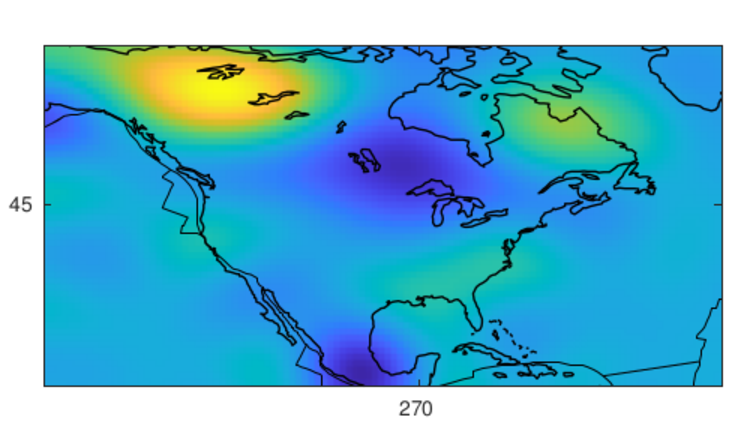
\includegraphics[scale=.75]{namerica_solvedcoefficients}
\end{figure}

For comparison, the Slepian function whose values are the entries in \verb!data! (that is, whose coefficients are the entries in \verb!lmcosi2coef(lmcosi,1)!) is graphed by

\verb!plotplm(lmcosi,[],[],4,1)!

\begin{figure}[H]
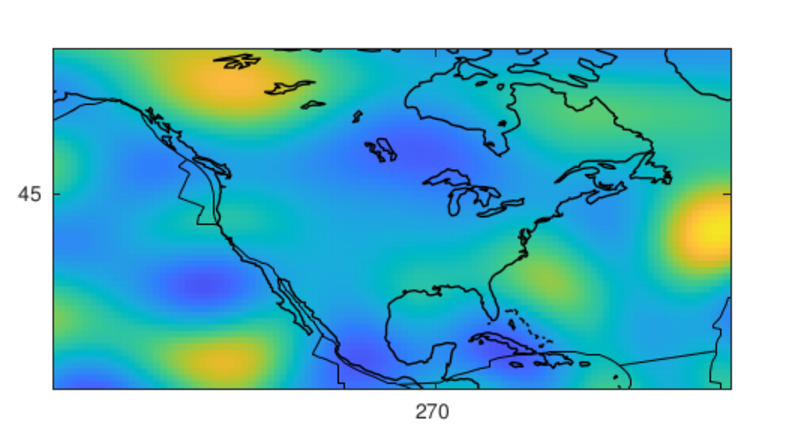
\includegraphics[scale=.75]{namerica_compare}
\end{figure}
 

\end{document}